\documentclass{article}
\usepackage{amsmath}
\usepackage{braket} % For Dirac notation
\usepackage{graphicx}
\usepackage{quantikz}
\usepackage{hyperref}
\usepackage{cleveref}

\usepackage[utf8]{inputenc}
\usepackage{geometry}
\usepackage{listings}
\usepackage{xcolor}

\usepackage{siunitx}
\usepackage{pgf}
\usepackage{subcaption}
\usepackage{float}

\geometry{a4paper, margin=1in}
\def\mathdefault#1{#1}

\definecolor{codegray}{rgb}{0.9,0.9,0.9}
\definecolor{bg}{rgb}{0.95,0.95,0.95}

\lstset{
  language=Python,                     % evidenziazione sintassi simile a Python
  basicstyle=\ttfamily\footnotesize,  % font più piccolo
  keywordstyle=\color{blue},          % stile per le parole chiave
  commentstyle=\color{gray},          % stile per i commenti
  stringstyle=\color{orange},         % stile per le stringhe
  breaklines=true,                    % manda a capo le righe lunghe
  breakatwhitespace=false,            % va a capo anche nel mezzo delle parole
  postbreak=\mbox{\textcolor{red}{$\hookrightarrow$}\space}, % simbolo dopo l'andata a capo
  frame=single,                       % riquadro attorno al codice
  rulecolor=\color{black},            % colore del bordo del riquadro
  captionpos=b,                       % posizione della didascalia in basso
  numbers=none,                       % niente numeri di riga
  numberstyle=\tiny\color{gray},      % stile dei numeri di riga (se attivati)
  numbersep=5pt,                      % distanza numeri-codice (se attivati)
  stepnumber=2,                       % numerazione ogni 2 righe (se attivati)
  firstnumber=1000,                   % inizia la numerazione da 1000
  xleftmargin=15pt,                   % margine sinistro
  keepspaces=true,                    % conserva spazi e indentazioni
  showspaces=false,                   % non mostra simboli per spazi
  showstringspaces=false,            % non sottolinea gli spazi nelle stringhe
  showtabs=false,                     % non mostra simboli per tab
  escapeinside={\%*}{*)},             % per inserire comandi LaTeX nel codice
  morekeywords={*,...},              % aggiunta di ulteriori parole chiave
  deletekeywords={...},              % rimozione di parole chiave predefinite
  backgroundcolor=\color{bg},        % colore di sfondo personalizzato
  title=\lstname                      % mostra il nome del file incluso (se usato)
}

\title{%
  {\Huge Quantum Hardware Design and Optimization} \\[0.5cm]
  {\LARGE Laboratory 1} \\
  {\large Quantum Gates Introduction}%
}

\author{}
\date{}

\begin{document}

\maketitle

\section{Evaluation by hand of the state evolution of a circuit}

\begin{figure}[h]

    \centering
\begin{quantikz}
\lstick{$\ket{0}$}   & \gate{H} \slice{$\ket{\psi_{t1}}$} & \ctrl{1} \slice{$\ket{\psi_{t2}}$} & \gate{H} \slice{$\ket{\psi_{t3}}$} & \gate{X}  \slice{$\ket{\psi_{t4}}$} & \ctrl{1} \slice{$\ket{\psi_{t5}}$} & \gate{X} \slice{$\ket{\psi_{t6}}$} & \gate{H} \slice{$\ket{\psi_{t7}}$} &  \meter{} \\
\lstick{$\ket{0}$}&\gate{H} & \gate{Z} & \gate{H} & \gate{X} & \gate{Z} & \gate{X} & \gate{H}& \meter{}
\end{quantikz}

    \caption{Circuit 1.}
        \label{fig:circuit_1}
\end{figure}
We are given the circuit in \cref{fig:circuit_1}. In the following we see the state of 
the circuit in each slice.
We start from the state
\begin{equation}
    \ket{\psi_0} = \ket{00}  \, .
\end{equation}
Then:
\begin{equation}
        \ket{\psi_1} = \ket{++} = \frac{1}{2} \left( \ket{00} + \ket{01} + \ket{10} + \ket{11} \right) = \sum_{n=0}^{3} \ket{n} \, ,
\end{equation}
\begin{equation}
        \ket{\psi_2} = \frac{1}{\sqrt{2}} \left( \ket{0+} + \ket{1-}\right) \, ,
\end{equation}
\begin{equation}
        \ket{\psi_3} = \frac{1}{\sqrt{2}} \left( \ket{+0} + \ket{-1} \right) \, ,
\end{equation}
\begin{equation}
        \ket{\psi_4} = \frac{1}{\sqrt{2}} \left( \ket{+1} - \ket{-0} \right)  \, ,
\end{equation}
Since CZ is symmetric:
\begin{equation}
        \ket{\psi_5} =  \frac{1}{\sqrt{2}} \left( \ket{-1} - \ket{-0} \right) =  - \ket{--} \, ,
\end{equation}
\begin{equation}
        \ket{\psi_6} = - \ket{--} \, ,
\end{equation}
\begin{equation}
        \ket{\psi_7} = - \ket{11} \, .
\end{equation}



\section{Quirk implementation}

To verify the correctness of the manual calculations, the circuit was recreated on the online platform \textbf{Quirk} (\url{https://algassert.com/quirk}).
The offline copy of the circuit can be opened by clicking the link below:
\href{run:es2.html}{Open the Quirk circuit offline}
From the \textit{State Vector Display} in Quirk, it can be observed that the final state of the system matches with the manually calculated result.


\section{Qiskit implementation}

The program defines a two-qubit quantum circuit with two classical bits for measurement. It begins by applying Hadamard gates to both qubits to create a superposition of states. A controlled-$Z$ gate is then applied to introduce a conditional phase shift and generate entanglement between the qubits. Throughout the circuit, Hadamard and Pauli-$X$ gates are alternated to manipulate the amplitudes and phases of the quantum state, controlling its evolution step by step. A controlled-NOT ($CX$) gate further couples the two qubits, enabling conditional transformations based on the state of the control qubit. The \texttt{barrier} instructions are included to visually separate logical sections of the circuit without affecting the computation. Finally, the qubits are measured and the results are stored in the corresponding classical bits, allowing observation of the output in the computational basis. The command \texttt{qc.draw('mpl')} displays the schematic of the circuit, as it can be seen in \cref{fig:qiskit circuit}.

\vspace{0.5cm}
\begin{lstlisting}[language=Python, caption={Qiskit code}, label={lst:qiskit-circuit}]
import qiskit
from qiskit import QuantumCircuit, transpile
from qiskit_aer import AerSimulator
from qiskit.visualization import plot_histogram
import matplotlib.pyplot as plt
from qiskit.qasm3 import dumps

# step 0: create a Quantum Circuit
qc = QuantumCircuit(2, 2)  # 2 qubits, 2 classical bits

# step 1:<
qc.h(0)
qc.h(1)

# step 2:
qc.cz(1, 0)

# step 3:
qc.h(0)
qc.h(1)

# step 4:
qc.x(0)
qc.x(1)

# step 5:
qc.cz(1, 0)

# step 6:
qc.x(0)
qc.x(1)

# step 7:
qc.h(0)
qc.h(1)

# measure q[0] -> c[0]; measure q[1] -> c[1];
qc.measure(0, 0)
qc.measure(1, 1)

qc.draw('mpl')  # draw circuit diagram
\end{lstlisting}





\begin{figure}[H]
    \centering
    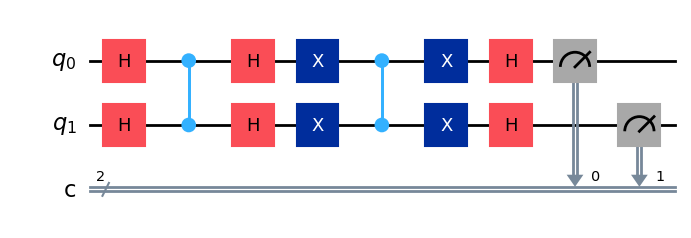
\includegraphics[width=0.7\textwidth]{images/circuit.png}
    \caption{Qiskit circuit}
    \label{fig:qiskit circuit}
\end{figure}


\begin{lstlisting}[language=Python, caption={Histogram with zero-count states}, label={lst:qiskit-hist}]
%matplotlib inline
from qiskit.visualization import plot_histogram

try:
    n_bits = len(next(iter(counts)))
except StopIteration:
    n_bits = getattr(qc, "num_qubits", 2)

labels = [format(i, f"0{n_bits}b") for i in range(2**n_bits)]
complete_counts = {b: counts.get(b, 0) for b in labels}

fig = plot_histogram(complete_counts, title="Measurements", bar_labels=True)
fig.show()
\end{lstlisting}

Through the previous code, the measurement results of the quantum circuit were visualized using a histogram, \cref{fig:output histogram}. The plot clearly shows that the only observed output is the bitstring \texttt{11}, while all other possible outcomes have zero probability. This indicates that the circuit deterministically evolves the quantum state into the final state $\ket{11}$, meaning that both qubits are measured in the state $\ket{1}$ with certainty.

\begin{figure}[H]
    \centering
    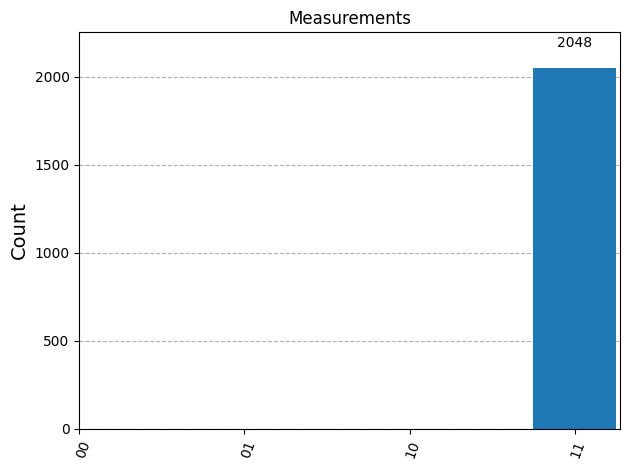
\includegraphics[width=0.7\textwidth]{images/histograms.png}
    \caption{output histogram}
    \label{fig:output histogram}
\end{figure}

%% Qasm 

The following two lines are used to convert the circuit into OpenQASM 3 code and display it:
\begin{lstlisting}[language=Python, caption={Export circuit to QASM3}, label={lst:qasm-export}]
qasm_str = dumps(qc)
print(qasm_str)
\end{lstlisting}

The first line serializes the circuit into QASM format, while the second prints the resulting code.

\begin{lstlisting}[language=Python, caption={Output generato: OpenQASM 3}, label={lst:qasm3-output}, backgroundcolor=\color{bg}]
OPENQASM 3.0;
include "stdgates.inc";
bit[2] c;
qubit[2] q;
h q[0];
h q[1];
cz q[1], q[0];
h q[0];
h q[1];
x q[0];
x q[1];
cz q[1], q[0];
x q[0];
x q[1];
h q[0];
h q[1];
c[0] = measure q[0];
c[1] = measure q[1];
\end{lstlisting}







\section{Optional}

\begin{figure}[h]
    \centering
\begin{quantikz}
\lstick{$\ket{0}$}   & \gate{H} \slice{$\ket{\psi_{t1}}$} & \ctrl{1} \slice{$\ket{\psi_{t2}}$} & \gate{H} \slice{$\ket{\psi_{t3}}$} & \gate{X}  \slice{$\ket{\psi_{t4}}$} & \qw & \ctrl{1} & \qw \slice{$\ket{\psi_{t5}}$} & \gate{X} \slice{$\ket{\psi_{t6}}$} & \gate{H} \slice{$\ket{\psi_{t7}}$} &  \meter{} \\
\lstick{$\ket{0}$}&\gate{H} & \gate{Z} & \gate{H} & \gate{X} &  \gate{H} & \targ{}  & \gate{H}  & \gate{X} & \gate{H}& \meter{}
\end{quantikz}

\end{figure}


\subsection{Evaluation by hand of the state evolution of a circuit}
Since we have that
\begin{equation}
    (I \otimes H) (CX_{1 \to 2}) ( I \otimes H) = CZ_{1 \to 2}
\end{equation}
The circuit is equivalent to the one we analyzed in section ... 

The demonstration is as follow: we check the action on a basis set: 
\begin{equation}
    \ket{0+}, \ket{0-}, \ket{1+}, \ket{1-}.
\end{equation}
The states with the control qubit set to $\ket{0}$ are unaltered, since $HH=I$, like in the $CZ_{1\to2}$. 
When the control qubit is set to $\ket{1}$, we have:
\begin{align}
    \ket{1+} \to \ket{1-} \\
    \ket{1-}  \to \ket{1+}.
\end{align}
Summarizing, te full action is:
\begin{align}
    \ket{0+} \to \ket{0+} \\
    \ket{0-}  \to \ket{0-} \\
    \ket{1+} \to \ket{1-} \\
    \ket{1-}  \to \ket{1+}.
\end{align}
And this is the exact action of the $CZ_{1 \to 2}$ gate in the circuit before.



The offline copy of the circuit can be opened by clicking the link below:
\href{run:es4_quirk.html}{Open the Quirk circuit offline}

\begin{lstlisting}[language=Python, caption={Qiskit code}, label={lst:qiskit-circuit}]
import qiskit
from qiskit import QuantumCircuit, transpile
from qiskit_aer import AerSimulator
from qiskit.visualization import plot_histogram
import matplotlib.pyplot as plt
from qiskit.qasm3 import dumps

# step 0: create a Quantum Circuit
qc = QuantumCircuit(2, 2)  # 2 qubit, 2 bit classici
# step 1:
qc.h(0)
qc.h(1)
qc.barrier(0, 1)
#step 2:
qc.cz(1, 0)

qc.barrier(0, 1)
# step 3:
qc.h(0)
qc.h(1)

qc.barrier(0, 1)
#stp 4:
qc.x(0)
qc.x(1)

qc.barrier(0, 1)
# step 5:
qc.h(1)

qc.barrier(0, 1)
# step 6:
qc.cx(0, 1)

qc.barrier(0, 1)
# step 7:
qc.h(1)

qc.barrier(0, 1)
# step 8:
qc.x(0)
qc.x(1)

qc.barrier(0, 1)
#step 9:
qc.h(0)
qc.h(1)

# measure q[0] -> c[0]; measure q[1] -> c[1];
qc.measure(0, 0)
qc.measure(1, 1)

qc.draw('mpl')        # diagramma grafico
\end{lstlisting}



\begin{figure}[H]
    \centering
    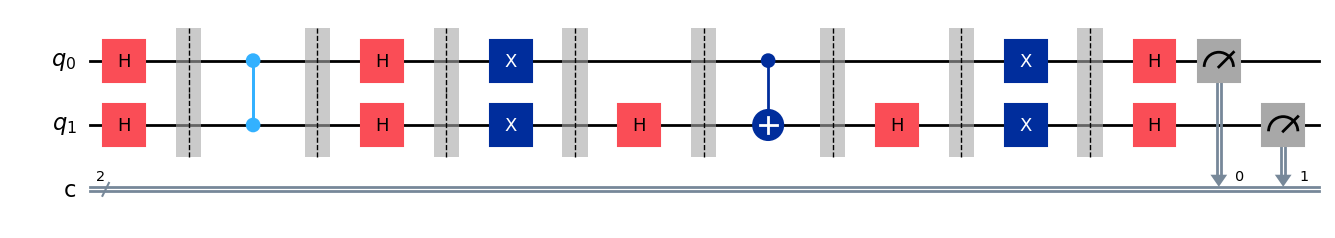
\includegraphics[width=1\textwidth]{images/circuit_es4.png}
    \caption{Qiskit circuit}
    \label{fig:circuit es4}
\end{figure}




%% Qasm 
\begin{lstlisting}[language=Python, caption={Export circuit to QASM3}, label={lst:qasm-export}]
qasm_str = dumps(qc)
print(qasm_str)
\end{lstlisting}

\begin{lstlisting}[language=Python, caption={Output generato: OpenQASM 3}, label={lst:qasm3-output}, backgroundcolor=\color{bg}]
OPENQASM 3.0;
include "stdgates.inc";
bit[2] c;
qubit[2] q;
h q[0];
h q[1];
barrier q[0], q[1];
cz q[1], q[0];
barrier q[0], q[1];
h q[0];
h q[1];
barrier q[0], q[1];
x q[0];
x q[1];
barrier q[0], q[1];
h q[1];
barrier q[0], q[1];
cx q[0], q[1];
barrier q[0], q[1];
h q[1];
barrier q[0], q[1];
x q[0];
x q[1];
barrier q[0], q[1];
h q[0];
h q[1];
c[0] = measure q[0];
c[1] = measure q[1];
\end{lstlisting}

\end{document}
